\renewcommand{\textfraction}{0.05} 
\documentclass[10pt, a4paper]{article}
\usepackage[portuguese]{babel}
\usepackage[utf8]{inputenc}
\usepackage[T1]{fontenc}
\usepackage{enumitem}
\usepackage{subfig}
\usepackage{tabularx}
\usepackage{cite}
\usepackage{amssymb}
\usepackage{mathtools}
\usepackage[]{algorithm2e}
\usepackage{graphicx}
\usepackage{tikz}
\usepackage{hyperref}
\usepackage{url}
\usetikzlibrary{positioning}

\graphicspath{ {images/} }

\begin{document}

\title{Desafio Técnico}

\author{Ricardo Yamamoto Abe}

\maketitle

\section{Introdução}

Este relatório é o resultado da análise dos dados de faturamento e
potencial de bairros do Rio de Janeiro, criação de modelos preditivos
e suas aplicações para fins de classificação e regressão para bairros
de São Paulo, além da segmentação por idade e classe social
relacionados ao público alvo.

\section{Pré-processamento}

Antes de carregar o arquivo csv no sistema, o cabeçalho foi alterado
para remover caracteres acentuados e cedilhas.

\subsection{Missing values}

Na primeira etapa de pré-processamento, foram detectados 2 problemas:

\begin{itemize}
\item Os bairros Eta Guaraú, Pico do Jaraguá e Reserva da Cantareira
  estavam com todos os totais de população por faixa etária e número
  de domicílios por classe zerados. Eles foram removidos da base.
\item Seis bairros do RJ não possuiam renda média: Anil, Catumbi,
  Freguesia, Jacaré, Rio Comprido e Maracanã. Essa coluna foi
  preenchida via \emph{MICE (Multiple Imputation by Chained
    Equations)}.
\end{itemize}

\subsection{Normalização de faixas etárias e total de domicílios}

Com o intuito de transformar as variáveis de faixa etária e domicílios
em números reais no intervalo $[0, 1]$, as colunas \texttt{popAte9,
  popDe10a14, popDe15a19, popDe20a24, popDe25a34, popDe35a49,
  popDe50a59} e \texttt{popMaisDe60} foram divididas pela população do
bairro, e as colunas \texttt{domiciliosA1, domiciliosA2, domiciliosB1,
  domiciliosB2, domiciliosC1, domiciliosC2, domiciliosD} e
\texttt{domiciliosE} foram divididas pelo total de domicílios do
bairro.

\subsection{Análise de \emph{outliers}}

Foram encontrados 2 bairros do Rio de Janeiro com dados identificados
como \emph{outliers} e que foram removidos da base:

\begin{itemize}
\item Campo Grande -- o \emph{dataset} indica população de 667 mil
  habitantes, mais que o dobro do segundo bairro mais populoso. Em
  2010, o total era de aproximadamente 328 mil pessoas.
\item Lagoa -- a renda média é superior a 63 mil Reais, praticamente o
  triplo do segundo bairro nesse quesito.
\end{itemize}

\subsection{Normalização para renda média e populaçào}

Para a normalização das colunas \texttt{rendaMedia} e
\texttt{populacao}, foram testadas duas funções: logaritmo e
\emph{standardization} ($\frac{X - \mu}{\sigma}$, basicamente deixando
a variável com média 0 e desvio padrão 1). 

A normalização via logratimo obteve melhor resultado na classificação
do potencial do bairro, enquanto que \emph{standardization} foi
superior para a regressão do faturamento.

\subsection{Redução da dimensionalidade}

Como ferramenta de redução de dimensionalidade, foi utilizada PCA
(Análise de Componentes Principais) na classificação do potencial do
bairro. Para regressão, optou-se por não utilizá-la.

Foram feitos alguns testes utilizando t-SNE (\emph{t-Distributed
  Stochastic Neighbor Embedding}), sem sucesso.

\section{Predição para São Paulo}

A estimativa de faturamento e potencial para cada bairro de São Paulo
encontram-se no arquivo \texttt{sp.csv}.

\subsection{Classificação do potencial do bairro}

O classificador utilizado para o potencial do bairro foi o XGBoost,
utilizando PCA e normalização da renda média e população por
logaritmo; sua acurácia na validação cruzada com 10 iterações foi de
86,61\%.

\subsection{Regressão para faturamento do bairro}

Para regressão do faturamento, foi utilizada a métrica R2, que pode
ser negativo para modelos arbitrariamente ruins, até 1.0, para um
modelo perfeito. Novamente foi utilizado XGBoost com renda média e
população normalizada via \emph{standardization}. O \emph{score}
obtido via validação cruzada de 10 iterações foi 0,8837.

\section{Segmentação}

Assumindo que o total de domicílios por classe econômica e a população
por faixa etária são variáveis independentes, podemos utilizar a
proporção de cada uma delas para calcular a probabilidade conjunta via
produto das marginais para cada um dos bairros. A segmentação foi
feita sobre as classes e idades do público alvo: 25 a 34 e 34 a 49
para idade; A1, A2, B1 e B2 para classes econômicas.

O algoritmo utilizado para encontrar os clusters foi o \emph{KMeans},
utilizando $k=9$, pois o processamento foi feito utilizando 2
proporções de idade e 4 de domicílio, totalizando 8 pares distintos;
uma classe a mais foi gerada para agrupar os bairros menos
interessantes do ponto de vista da pesquisa.

\begin{figure}[]
\centering
\begin{tabular}{cc}
\subfloat[]{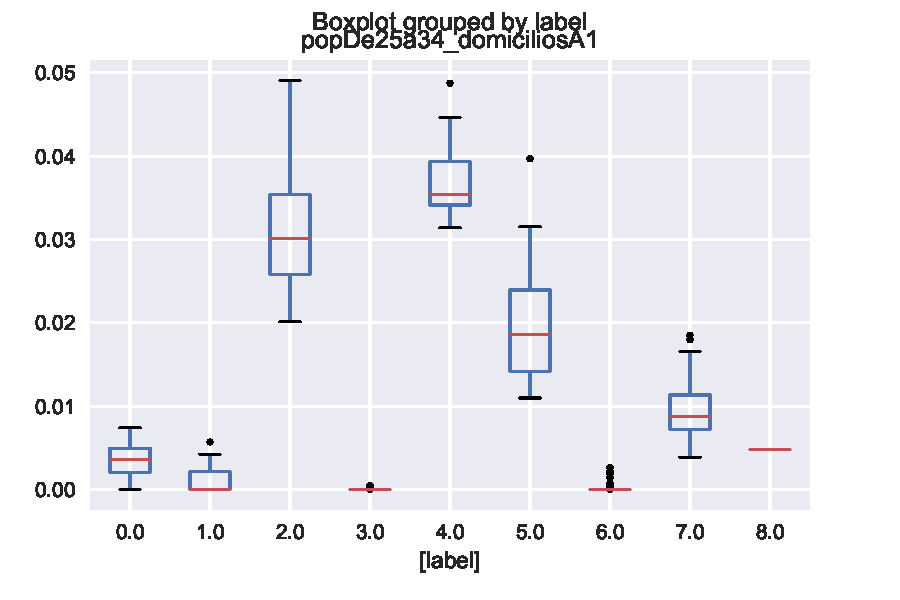
\includegraphics[scale=0.4]{pop2534a1.pdf}} 
\subfloat[]{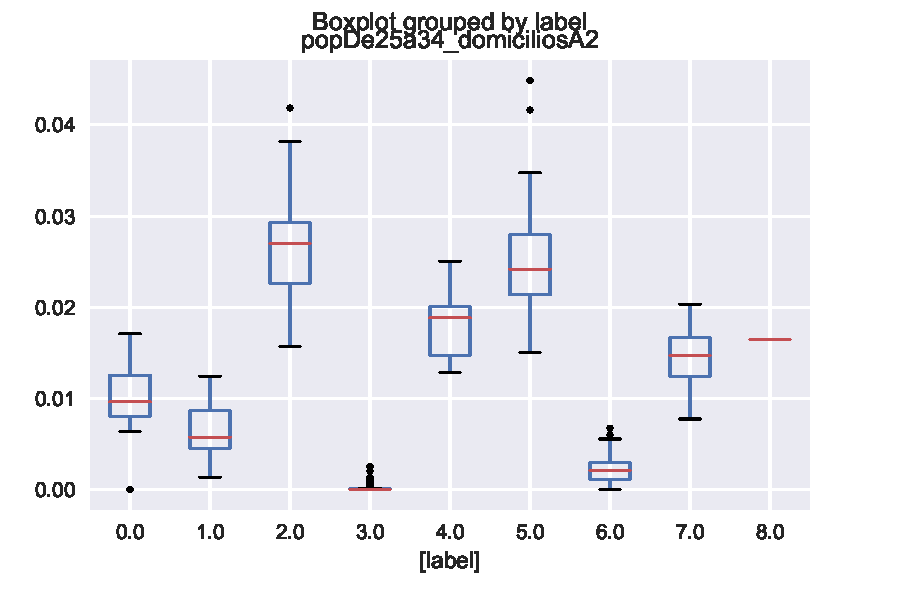
\includegraphics[scale=0.4]{pop2534a2.pdf}}  
\\
\subfloat[]{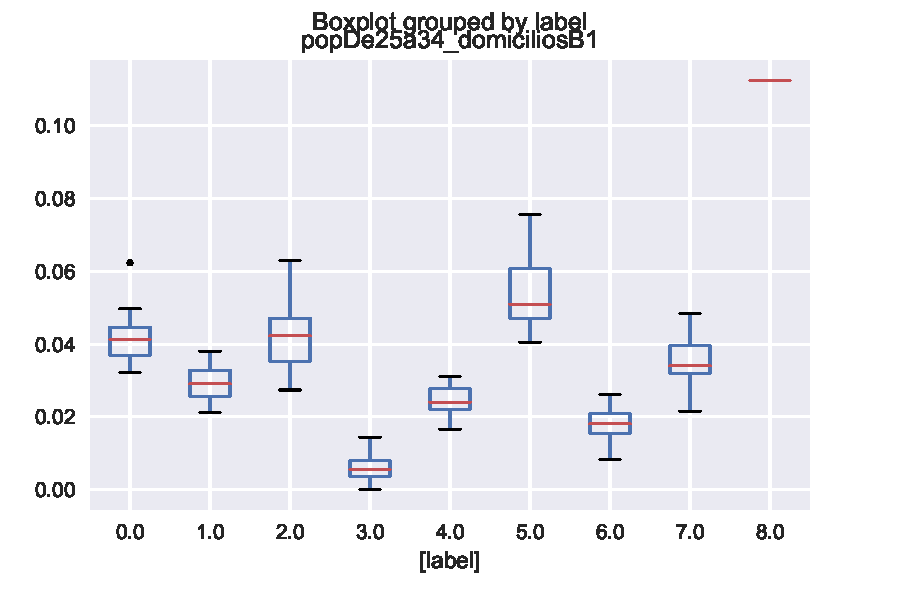
\includegraphics[scale=0.4]{pop2534b1.pdf}} 
\subfloat[]{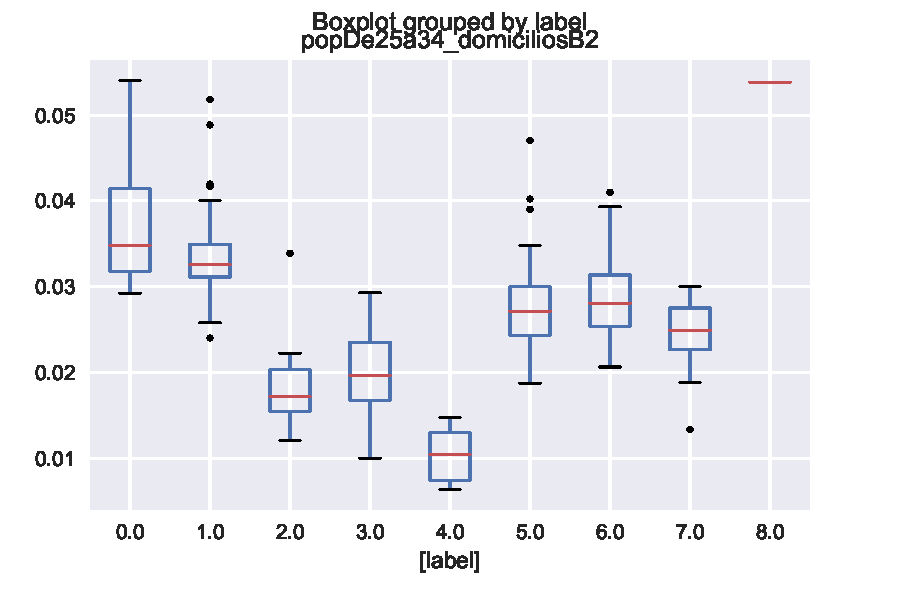
\includegraphics[scale=0.4]{pop2534b2.pdf}}  
\\
\subfloat[]{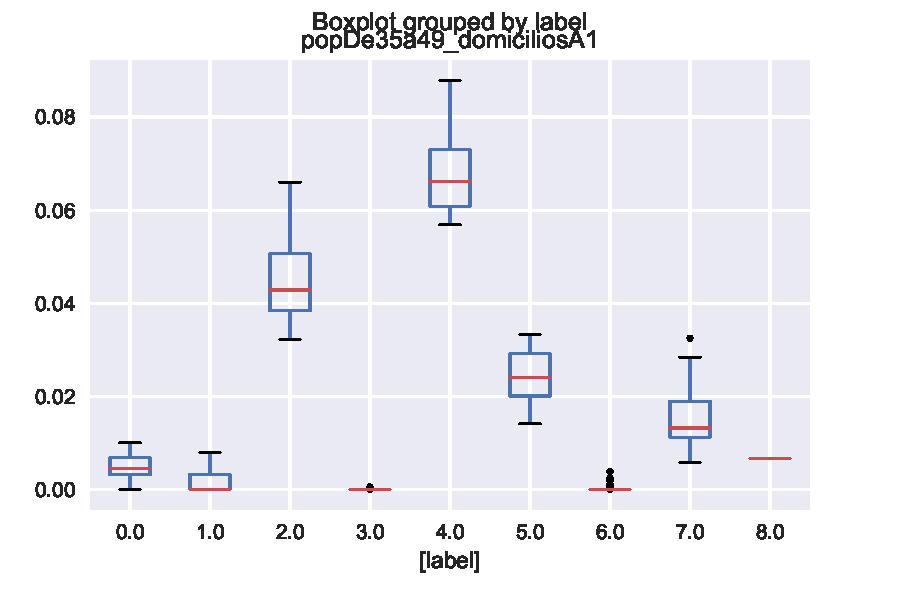
\includegraphics[scale=0.4]{pop3549a1.pdf}} 
\subfloat[]{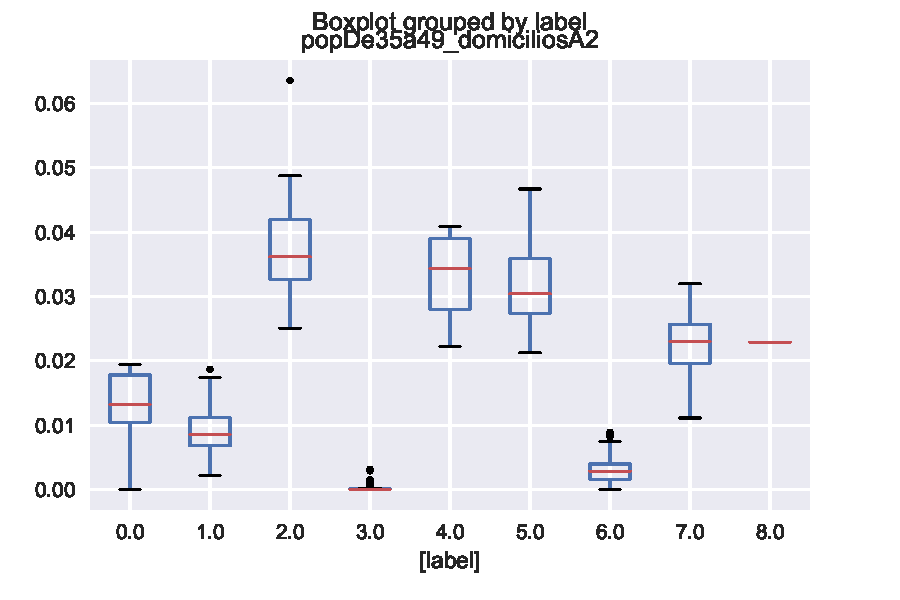
\includegraphics[scale=0.4]{pop3549a2.pdf}}  
\\
\subfloat[]{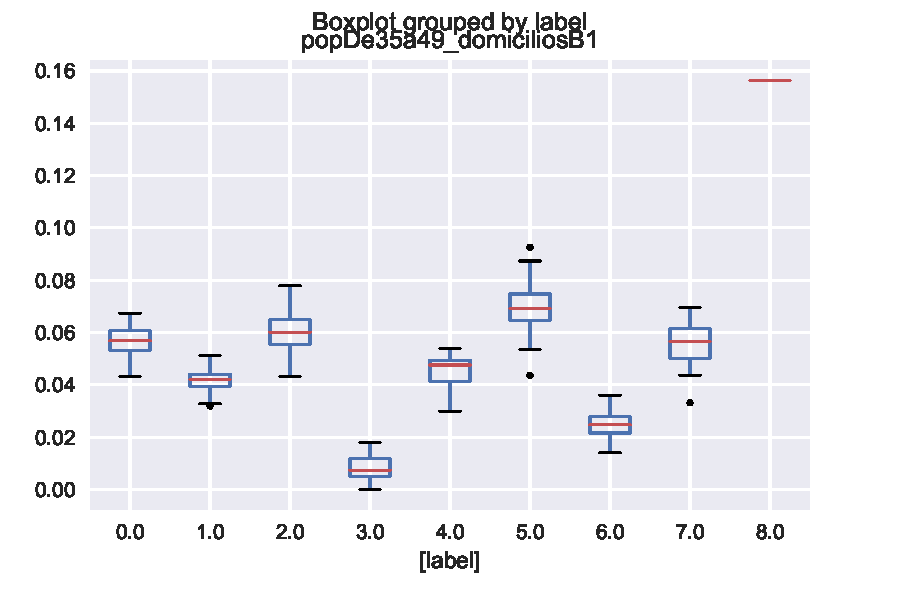
\includegraphics[scale=0.4]{pop3549b1.pdf}}
\subfloat[]{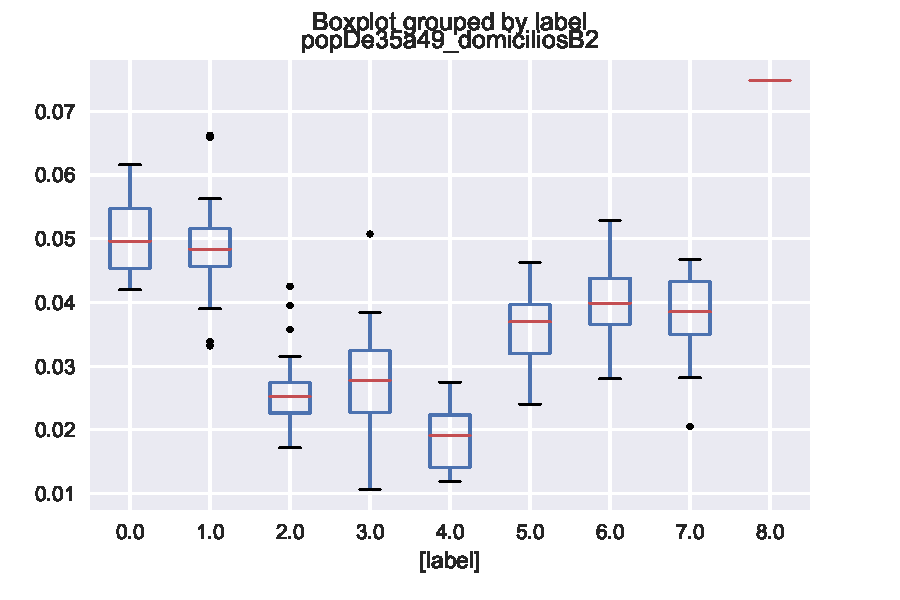
\includegraphics[scale=0.4]{pop3549b2.pdf}}
\end{tabular}
\caption{Boxplots agrupados por label de cada cluster}
\label{fig:segmentacao}
\end{figure}

\begin{figure}[]
\centering
\begin{tabular}{c}
\subfloat[]{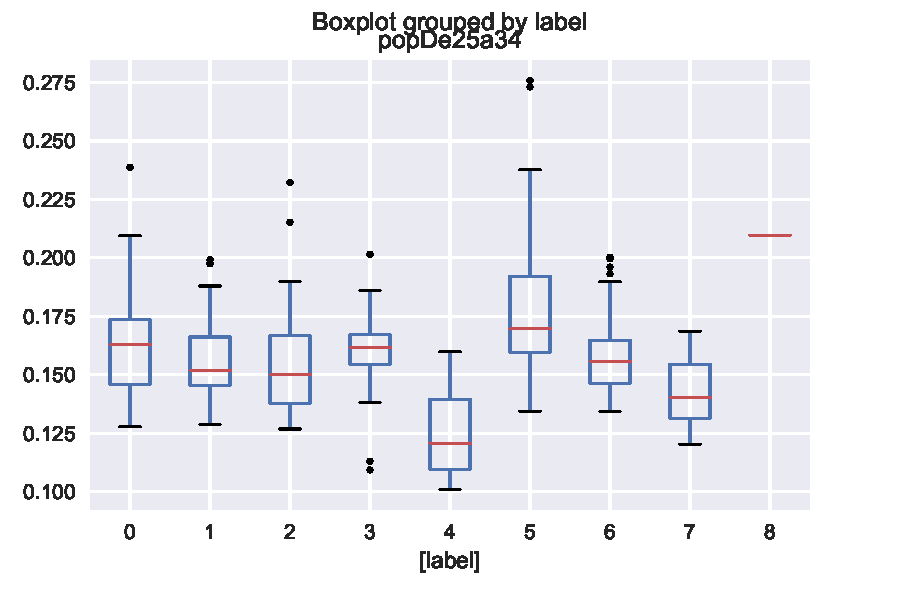
\includegraphics[scale=0.6]{pop2534.pdf}} 
\\
\subfloat[]{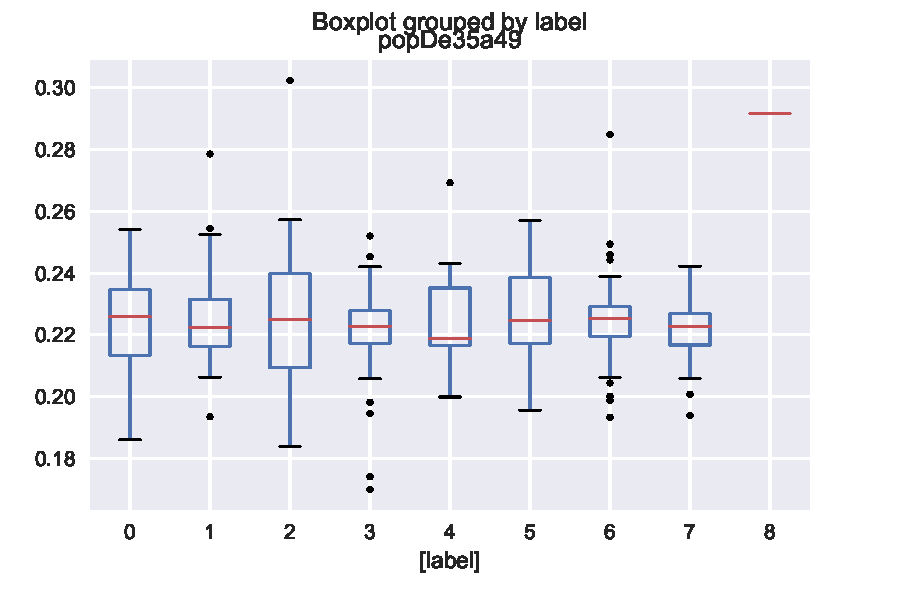
\includegraphics[scale=0.6]{pop3549.pdf}}  

\end{tabular}
\caption{Boxplots das faixas etárias 25 a 34 e 35 a 49 para clusters
  de São Paulo}
\label{fig:faixas_etarias}
\end{figure}

Foi feita uma tentativa de clusterização via HDBSCAN, mas os
resultados não foram bons.

Na figura \ref{fig:segmentacao}, encontramos os seguintes boxplots:

\begin{enumerate}[label=(\alph*)]
\item População de 25 a 34 anos, classe A1
\item População de 25 a 34 anos, classe A2
\item População de 25 a 34 anos, classe B1
\item População de 25 a 34 anos, classe B2
\item População de 34 a 49 anos, classe A1
\item População de 34 a 49 anos, classe A2
\item População de 34 a 49 anos, classe B1
\item População de 34 a 49 anos, classe B2
\end{enumerate}

Analisando os boxplots, encontramos a seguinte segmentação:

\begin{itemize}
\item Cluster 0 -- representatividade na classe B2, para ambas as
  faixas de idade.
\item Cluster 1 -- representatividade na classe B2 (menor que no
  cluster 0), para ambas as faixas de idade.
\item Cluster 2 -- representatividade nas classes A1 e A2, para ambas
  as faixas de idade.
\item Cluster 3 -- é o cluster onde os bairros menos interessantes
  para investimento.
\item Cluster 4 -- é o cluster com maior proporção de domicílios na
  classe A1, para ambas as faixas de idade, mas pela análise da
  marginal popDe25a34 (figura \ref{fig:faixas_etarias}), abaixo de
  todas os outros clusters, parece ser mais aderente à faixa de idade
  35-49.
\item Cluster 5 -- representatividade nas classes B1 e A2, para ambas
  as faixas de idade. Também é relevante para a classe A1 em ambas as
  faixas de idade.
\item Cluster 6 -- representatividade em B2, para ambas as faixas de
  idade.
\item Cluster 7 -- representação equilibrada entre todas as classes
  econômicas e faixas de idade.
\item Cluster 8 -- o bairro do Parque Anhembi, tem uma proporção acima
  do esperado nas classes B1 e B2, para ambas as faixas de idade.
\end{itemize}

Os arquivos com os bairros separdos por segmentos são:
\texttt{segment\_00.csv}, \texttt{segment\_01.csv}, \dots,
\texttt{segment\_08.csv}.

\section{Outras bases de dados}

Para este projeto, imagino que os dados de pesquisa origem-destino do
metrô de SP (feito em 2017, dado público) e do plano diretor de
transporte urbano do RJ (2002/2003, dado público, mas aparentemente
faltam as planilhas com mais detalhes dos dados) serviriam para
indicar não só onde as pessoas moram, mas também quais seus outros
pontos de interesse: trabalho, estudo e lazer. Assim sendo, uma pessoa
do público alvo poderia ser observada não apenas em sua moradia, mas
em locais prováveis para onde ela vai.

A API do Google Places (dado privado) e a base da wikimapia (dado
público) poderiam ser utilizados para indicar estabelecimentos
comerciais já existentes para analisar prováveis concorrentes em um
determinado bairro.

\end{document}





